\chapter{\textbf{Methodology}} \label{cap:methodology}

The traditional approach in terms of economic sentiment is the construction of sentiment indices through surveys \cite[p.4]{shapiro2020measuring} -- ``Usually, these surveys are monthly, with interviews and even verification of the interviewees' personal finances'' \cite[p. 5]{shapiro2020measuring}. The idea of this work is to obtain a sentiment index through sentiment analysis and Natural Language Processing techniques.

\section{Natural Language Processing}

According to \cite{liddy2001natural}, Natural Language Processing (NLP) is a computational approach to textual analysis that is based on both a set of theories and a set of technologies. In other words, by the formal definition, ``Natural Language Processing is a theoretically motivated range of computational techniques for analyzing and representing naturally occurring texts at one or more levels of linguistic analysis for the purpose of achieving human-like language processing for a range of tasks or applications'' \cite[p. 2]{liddy2001natural}. The purpose of this tool is, therefore, ``to accomplish human-like language processing''. In general, the classification of a text, phrase, or even word is given categorically according to its positivity (positive, negative, neutral), or through valence scores, from 1 to 5. ``The sentiment of text is a measure of the speaker's tone, attitude, or evaluation of a topic, independent of the topic's own sentiment orientation (e.g., a horror movie can be `delightful')'' \cite[p. 5]{shapiro2020measuring}.\\

The present work will use lexical-based NLP techniques. ``At this level, humans, as well as NLP systems, interpret the meaning of individual words. Several types of processing contribute to word-level understanding – the first of these being assignment of a single part-of-speech tag to each word. In this processing, words that can function as more than one part-of-speech are assigned the most probable part-of-speech tag based on the context in which they occur'' \cite[p.7]{liddy2001natural}. Still, ``Additionally at the lexical level, those words that have only one possible sense or meaning can be replaced by a semantic representation of that meaning. The nature of the representation varies according to the semantic theory utilized in the NLP system. The following representation of the meaning of the word launch is in the form of logical predicates. As can be observed, the single lexical unit is decomposed into its more basic properties. Given that there is a set of semantic primitives used across all words, these simplified lexical representations make it possible to unify meaning across words and to produce complex interpretations, much the same as humans do'' \cite[p.7]{liddy2001natural}.\\

\section{Sentiment Analysis and Lexicons}

In the scope of sentiment analysis, it is necessary to use a dictionary of sentiments to detect polarities of sentiments and positive/negative scores. From the scores and polarities, it is possible to obtain a sentiment index that generates a possible correlation with the macroeconomic scenario. Basically, a sentiment dictionary works by indicating a specific punctuation for each word, taking into account punctuation and connectives. That is, depending on how a sentence or sentence is written, its polarity (score) varies.\\


\subsection{Sentiment Lexicons} \label{sec:lexicons}
One of the most adopted and valuable resources for sentiment analysis is the use of sentiment lexicons \cite[]{ahire2014survey, nusko2016building, cambria2013new, kaity2020sentiment}. A sentiment lexicon is a collection of words (sometimes referred to as polar or opinion words) linked to their sentiment orientation, that is, positive or negative \cite[]{kaity2020sentiment, medhat2014sentiment}.


\subsection{Polarity-based Lexicons} \label{subsec:polbas}

Polarity-based Lexicons are lexicons that allow you to automatically evaluate a text based on its polarity. These lexicons are ``a basic resource for analyzing the sentiments and opinions expressed in texts'' \cite[p.938]{san2016polarity}. When analyzing a text from the perspective of sentiment analysis, a polarity-based lexicon, words and phrases are commonly classified as positive, neutral and negative. If we take the example of the phrase ``Good people sometimes have bad days'', a polarity-based lexicon would possibly classify the word ``Good'' being a \textit{positive} word and the word ``bad'' would probably be classified as \textit{negative} -- the other words in the sentence would possibly be classified as ``neutral'' \cite[]{BCDG07}.\\

In terms of score classification, \cite{BCDG07} shows that in proportional and popular values a positive score can be presented as:
\begin{align*}
score = \frac{\text{number of positive words - number of negative words}}{\textit{number of positive words + number of negative words}}
\end{align*}

where \textit{number of positive words} would be the total number of positive words in a sentence or text and \textit{number of negative words} would be the total number of negative words in a sentence or text.\\

A possible barrier observed is in relation to the elaboration of a polarity-based lexicon and the way in which a lexicon is created \cite[]{stone1966general}. The vast majority of polarity-based lexicon is aimed at generic texts (without a specificity) -- when extracting sentiments from specific texts (such as economic and financial) a lexicon could present spurious results for not taking into account words that in the economic field can be considered positive or negative (the vast majority of lexicons do not include words and economic terms such as ``inflation'', ``recession'', or other such terms) \cite[]{loughran2011liability}.\\

\begin{table}[!h]
\caption{Examples of polarities in a polarity-based lexicon -- LM-SA-2020}
\adjustbox{max width=\textwidth}{
\begin{tabular}{ll|ll|ll|ll}
\hline
Word       & Polarity & Word        & Polarity & Word          & Polarity & Word        & Polarity \\ \hline
Abundance  & Positive & Abandon     & Negative & Inspirational & Positive & Defensive   & Negative \\
Abundant   & Positive & Abdicated   & Negative & Invented      & Positive & Dever       & Negative \\
Acclaimed  & Positive & Abdicates   & Negative & Inventor      & Positive & Deficit     & Negative \\
Accomplish & Positive & Aberrant    & Negative & Leadership    & Positive & Defraud     & Negative \\
Advances   & Positive & Aberrations & Negative & Leading       & Positive & Defunct     & Negative \\
Achieves   & Positive & Abrupt      & Negative & Lucrative     & Positive & Degradation & Negative \\ \hline
\end{tabular}
}
\caption*{Source: Words and polarities taken from \cite[]{lmdata}}
\label{tab:polarity}
\end{table}

Table \ref{tab:polarity} presents examples of a lexicon based on polarities. Note, however, that this lexicon was constructed based on economic terms and words, based on over 10,000 economic and financial articles \cite[p.1]{lmdata}.\\

In general, when a polarity-based lexicons is applied to a text, more advanced computational techniques are not necessary, except for an interactive algorithm that computes the polarity of the text \cite[]{BCDG07}. 

\subsection{Valence-based Lexicons}

A valence-based lexicon can be justified by the need that when analyzing a text or phrase the expected results can be not only binary (positive and negative), but determined by the ``intensity'' of each word or phrase \cite[] {hutto2014vader}. When considering a valence-based lexicon, polarity is the main focus in determining the scores of \cite[]{cambria2012senticnet} words and texts. The authors develop a valence-based lexicon so that texts and words have values such that the $score_i$ (with $i$ being a word, text or even phrase) ranges from $-1$ to $1$, so that $ score_i \subset (-1, 1) \quad \forall \quad score_i \in \mathbb{R}$.\\

Even though \cite{cambria2020senticnet} is a valence-based lexicon implemented in Python, compared to other valence-based lexicons \cite[]{hutto2014vader} gives inferior results to other valence-based lexicon.


\subsection{VADER – Valence Aware Dictionary for sEntiment Reasoning} \label{subsec:vader}

VADER, or Valence Aware Dictionary for sEntiment Reasoning is a lexicon initially created as a parsimonious lexicon for social media text. However, it has been used in general cases of textual sentiment analysis given it's benchmarks compared to other lexicons or even machine learning oriented techniques ``relying on Naive Bayes, Maximum Entropy, and Support Vector Machine (SVM) algorithms'' \citep[p.216]{hutto2014vader}. Differently of most part of lexicons, VADER was created taking into account a combination of qualitative and quantitative methods to empirically validates and produces a \textit{golden-standard} sentiment lexicon \cite{hutto2014vader}.\\

Due to the fact that VADER is an open-source lexicon, it is relatively simple to modify -- even if it is not what was done in this work, it would be possible, if necessary, merging VADER with some other lexicons, with the objective of creating a more complex and dense lexicon focused on economic science and finance. This lexicon has about 7520 words and textual forms with a classified score compound which after normalized varies from -1 to 1 such that:
\begin{align} \label{eq:vaadercoumpond}
    score_ = \begin{cases}
                positive\quad if \quad compound > 0.05\\
                neutral\quad if \quad 0.05 \geq compound \geq -0.05\\
                negative\quad if \quad compound < 0.05
              \end{cases} \qquad \forall\quad compound \in (-1, 1)
\end{align}

The positive, neutral and negative scores are ratios for each category that the text or expression fells on: 
\begin{quote}
    ``These are the most useful metrics if you want to analyze the context \& presentation of how sentiment is conveyed or embedded in rhetoric for a given sentence. For example, different writing styles may embed strongly positive or negative sentiment within varying proportions of neutral text -- i.e., some writing styles may reflect a penchant for strongly flavored rhetoric, whereas other styles may use a great deal of neutral text while still conveying a similar overall (compound) sentiment. As another example: researchers analyzing information presentation in journalistic or editorical news might desire to establish whether the proportions of text (associated with a topic or named entity, for example) are balanced with similar amounts of positively and negatively framed text versus being "biased" towards one polarity or the other for the topic/entity'' \cite{vadergit}.
\end{quote}

Even when VADER excels when in social media, it's scores benchmarks when considered newspaper editorials are higher above the other lexicons or machine learning techniques (Table \ref{tab:vaderscore}) -- ``Surprisingly, when we further inspect the classification accuracy, we see that VADER (F1 = 0.96) actually even outperforms individual human raters (F1 = 0.84) at correctly classifying the sentiment of tweets into positive, neutral, or negative classes'' \citep[p.216]{hutto2014vader}.

\begin{table}[!h]
\centering
\caption{VADER 3-class classification performance as compared to individual human raters and 7 established lexicon baselines}
\begin{tabular}{l|c|c|c|c}
\hline
\multicolumn{2}{l|}{Correlation to ground truth} & \multicolumn{3}{l}{Classification Accuracy Metrics}   \\ \cline{3-5} 
\multicolumn{2}{l|}{(mean of 20 humans raters)}  & Overall Precision & Overall Recall & Overall F1 score \\ \hline
\multicolumn{5}{c}{NY Times Editorials (5,190 article snippets)}                                         \\ \hline
Ind. Humans                & 0.745               & 0.87              & 0.55           & 0.65             \\
VADER                      & 0.492               & 0.69              & 0.49           & 0.55             \\
Hu-Liu04                   & 0.487               & 0.70              & 0.45           & 0.52             \\
SCN                        & 0.252               & 0.62              & 0.47           & 0.38             \\
GI                         & 0.362               & 0.65              & 0.44           & 0.49             \\
SWN                        & 0.262               & 0.57              & 0.49           & 0.52             \\
LIWC                       & 0.220               & 0.66              & 0.17           & 0.21             \\
ANEW                       & 0.202               & 0.59              & 0.32           & 0.35             \\
WSD                        & 0.218               & 0.55              & 0.45           & 0.47             \\ \hline 
\end{tabular}
\caption*{Source: \citep[p. 223]{hutto2014vader}}
\label{tab:vaderscore}
\end{table}

\subsection{Loughran-McDonald: LM-SA-2020}  \label{subsec:loughran}

The other lexicon used in this work is the LM-SA-2020 and was the same provided by \cite{loughran2011liability}. Fundamentally, the difference between this one is the composition: the authors developed a dictionary with the purpose of revising the traditional lexicons in which certain words are or are not considered positive or negative in the economic and financial sphere \citep[p. 35]{loughran2011liability}:

\begin{quote}
    ``The motivation for building the LM-SA-2020 word list was based on an experiment using the above-mentioned original lists to detect sentiment-carrying words in South African financial article headlines''\citep[p. 1]{lmdata}
\end{quote}

This lexicon uses 808 financial articles and only about 37\% of the headlines actually corresponded to the expected sentiments (either in terms of words or expressions) given the articles verified by the authors\citep{loughran2011liability}. In terms of benchmark, with adding economic words and removing others in terms of polarity, sentiment detection and prediction increased by about 29\% when added to NLTK's WordNet\footnote{\url{https://www.nltk.org/howto/wordnet.html}}.\\

The results obtained by the authors were based on an analysis of two samples of reference articles: first, the authors considered a sample of 10 thousand files related to firms subject to shareholder litigation under Rule 10b-5. The other sample used by the authors considers \cite{doyle2007accruals}, between August 2002 and November 2005, companies disclosed at least one material deficiency in internal control \citep[p. 41]{loughran2011liability}. The authors estimated different models\footnote{In fact, 28 different Logit models were estimated. The economic variables used were The number of shares outstanding times the price of the stock as reported by CRSP on the day before the file date; Book-to-market (Derived from the Compustat and CRSP data items as specified in Fama and French (2001). The variable is based on the most recent Compustat data no more than 1 year before the file date. After eliminating observations with negative book-to-market, we winsorize the book-to-market variable at the 1\% level); The volume of shares traded in days [−252, −6] prior to the file date divided by shares outstanding on the file date. At least 60 observations of daily volume must be available to be included in the sample; The prefile date Fama–French alpha based on a regression of their three-factor model using days [−252, −6]. At least 60 observations of daily returns must be available to be included in the sample; The percent of institutional ownership reported in the CDA/Spectrum database for the most recent quarter before the file date. The variable is considered missing for negative values and winsorized to 100\% on the positive side; The average volume of the 4-day event window [0, 3], where volume is standardized based on its mean and standard deviation from days [−65, −6]; The root-mean square error from a Fama–French three-factor model for days [6, 252], with a minimum of 60 daily observations; Standardized unexpected earnings for the quarterly earnings announced within 90 days after the 10-K file date. The actual earnings and the analyst forecast consensus (mean) are from I/B/E/S unadjusted files, which are used to avoid the rounding issue. The unexpected earnings are standardized with stock price; The standard deviation of analysts’ forecasts in the most recent period prior to the earnings announcement used to calculate SUE, scaled by the stock price at the end of the quarter; The monthly change in the mean of analysts’ forecasts, scaled by the stock price in the prior month; and a dummy variable set equal to one for firms whose shares are listed on the NASDAQ stock exchange, else zero\citep[p.63]{loughran2011liability}} to reach the final conclusion that the lexicon accuracy increases with the addition or change of economic terms.\\

The lexicon created by the authors also allows for a more comprehensive classification in which, in addition to classifying certain words and terms as positive and negative, it also classifies them as ``uncertainty, litigious, strong modal, and weak modal words''\citep[p.62]{loughran2011liability}: 
\begin{quote}
    ``The paper finds evidence that some word lists are related to market reactions around the 10-K filing date, trading volume, unexpected earnings, and subsequent stock return volatility. [\dots] we show that financial researchers should be cautious when relying on word classification schemes derived outside the domain of business usage. Applying nonbusiness word lists to accounting and finance topics can lead to a high misclassification rate and spurious correlations''\citep[p.62]{loughran2011liability}
\end{quote}

\section{Procedure and Cross Validation}

In terms of organizational and methodological structure of the work, lexicons are used in the initial process in order to process the texts as a whole and extract the index of feelings.\\

As an initial procedure, the first necessary methodology input is the ECB speeches. A textual corpus is created from the discourses -- a corpus can be defined as a database that contains a set of texts, each with its respective Id for organizational purposes. In this work, the corpus used has, in addition to Id and texts, a column of dates, referring to the temporal moment of each discourse. With this database, a lexicon reading algorithm is applied to the texts and the referring feelings are extracted when in relation to the VADER and LM-SA-2020 lexicons in order to obtain the referring values for the sentiment variables.\\

The other necessary methodological input refers to the economic variables: from the dataset obtained from the corpus, it is necessary to merge these data with the economic variables in order to obtain, again, a new dataset. The last step in the data manipulation and organization process is data wrangling -- data wrangling is the process of altering and mapping data to make it more suitable and valuable for various downstream applications such as analytics \cite[]{dplyr2022, wickham2016r}. In this part of the process, operations to treat missing values and outliers were used, so that the obtained database is ``clean'' and usable for statistical and econometric modeling.\\

Finally, the last part of the methodological process is the part referring to econometric modeling and the so-called Cross Validation procedure. Cross Validation is a technique widely described in the literature \cite[]{hoornweg2018science, hastie2009elements, stone1974cross, breiman1992submodel} that aims to obtain optimal parameters from a predefined model. In Cross Validation, the dataset is divided between a training dataset and a test dataset, these being composed of 80\% and 20\% of the original dataset \cite[291]{breiman1992submodel}. The model, then, ``is estimated with a training sample and these estimates are used to ‘predict’ the outcomes of the validation sample. By varying the choice of a tuning parameters, one can select the set of configurations that leads to the best pseudo-out-of-sample forecasts''\cite[p.136]{hoornweg2018science}.\\

That said, this same methodology was used: from the clean database obtained, it is divided into a Train dataset and a Test dataset so that the Train dataset is used to obtain the best estimated model -- iteratively, several models are estimated and then the best one is selected from the metric evaluation criteria. Computationally, this can be the most time-consuming part of the process depending on both the number of iterations needed to obtain the best model, and the parameters and variables used. When the best model is obtained, it is then estimated from the Test dataset and the results and model accuracy are extracted.\\

Figure \ref{fig:diagram} presents the organizational diagram of the project. Details about the estimated models can be found in Chapter \ref{cap:results}: in order to present the necessary mathematical and statistical foundations, the models estimated in this work (LASSO, Adaptive LASSO, Elastic Net and VAR) all go through the Cross Validation and are chosen according to the metric evaluation measures adopted. Figure \ref{fig:diagram} presents the organizational diagram of the project. Details about the estimated models can be found in Chapter \ref{cap:results}: in order to present the necessary mathematical and statistical foundations, the models estimated in this work (LASSO, Adaptive LASSO, Elastic Net and VAR) all go through the Cross Validation and are chosen according to the metric evaluation measures adopted. \\



\begin{landscape}
\begin{figure}
    \centering
    \caption{Diagram of the Methodology Used}
    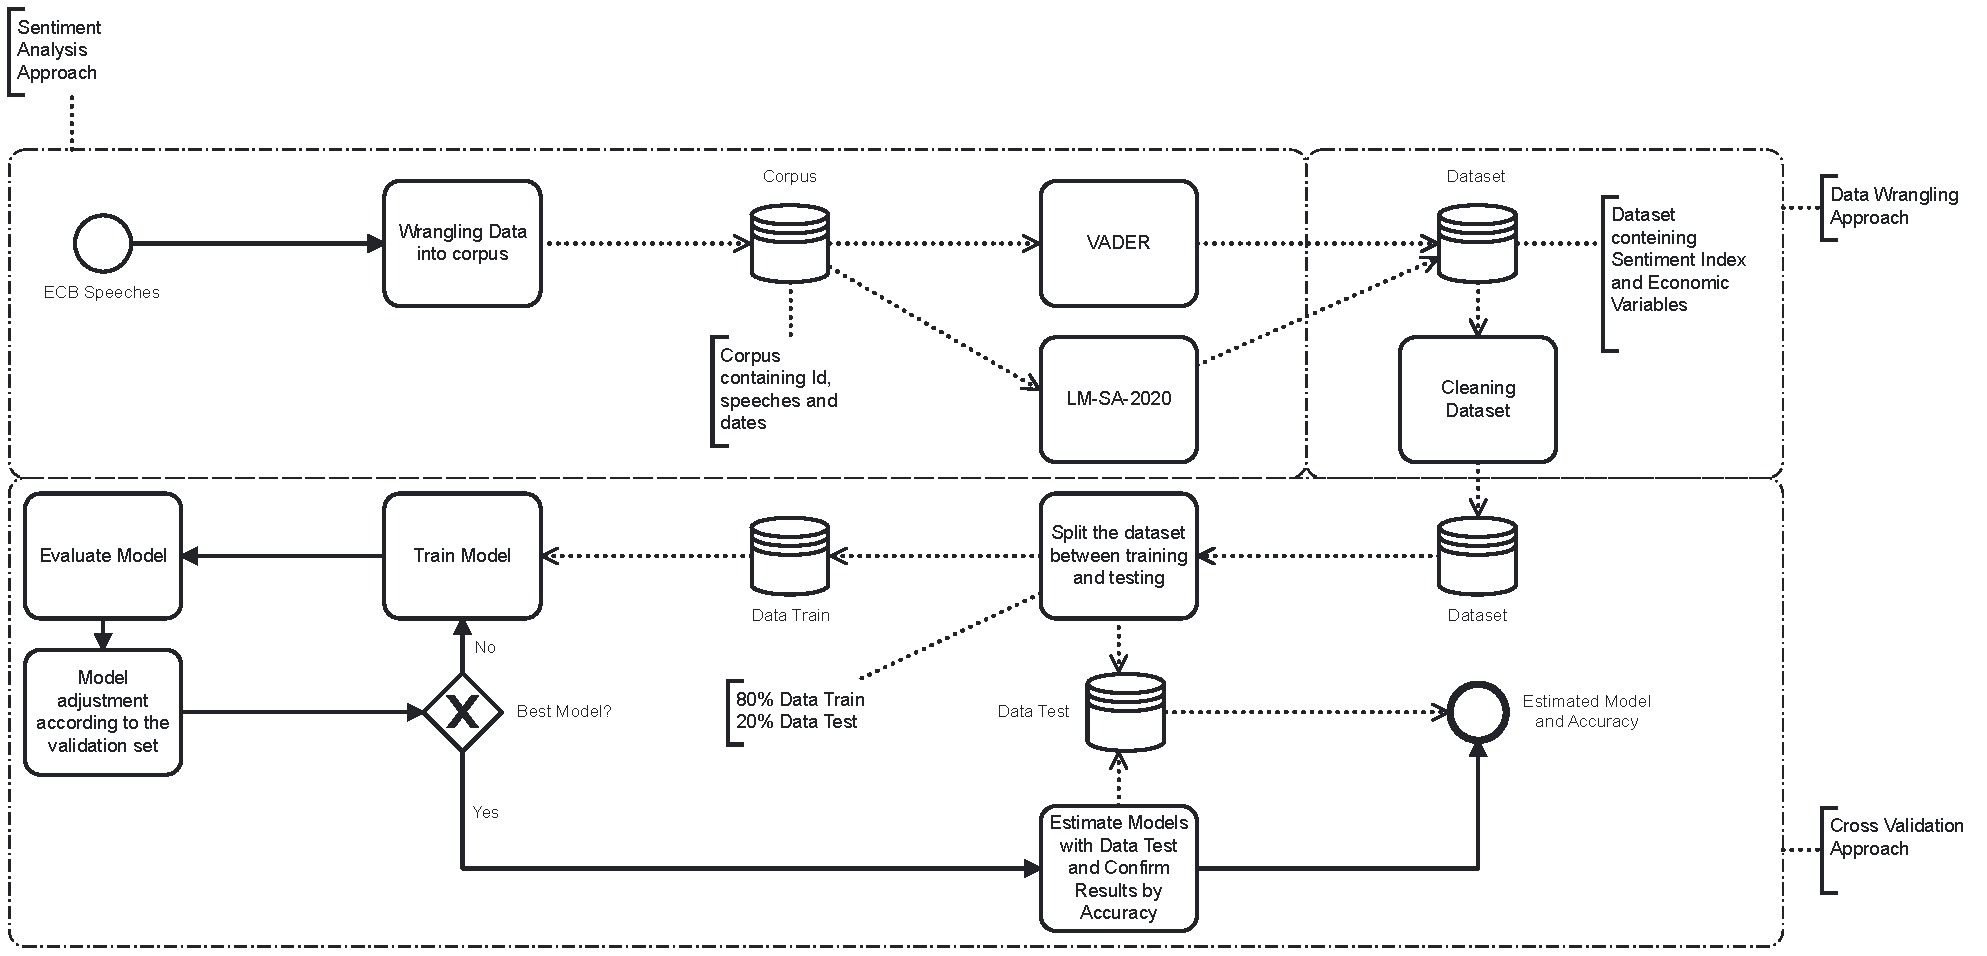
\includegraphics[width = \linewidth]{images/diagram.pdf}
    \caption*{Note: the procedure described in the flowchart defines the evolution of the project in order to describe the general procedures used. For information about the databases used, the \href{https://github.com/gustavovital/Dissertation/tree/main/data}{database repository} is free to consult}
    \label{fig:diagram}
\end{figure}
\end{landscape}


%\begin{figure}[!h]
%    \centering
%    \caption{Cross Validation Flowchart}
%    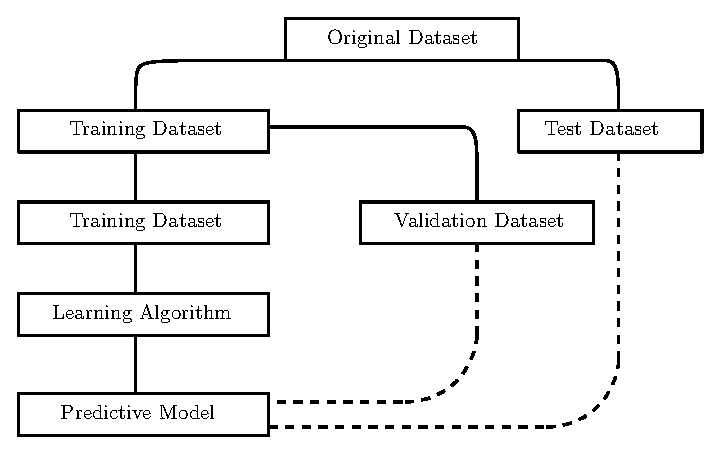
\includegraphics[width=.6\textwidth]{images/validation.eps}
%    \label{fig:cv}
%\end{figure}





%\section{Vector Autoregressive} \label{sec:var}


